% ============================================================
% Manuscript prose pass -- local mirror for Overleaf paste-in
% 2026-08-25
% ============================================================
% This follows the consistency-and-integration plan you reviewed, WITH
% ONE ADJUSTMENT: Figure 3 stays the CURRENT 3-panel main-text figure
% (fig3_regimes.R: A = locked recovery, B = shock across the feedback-
% strength grid, C = history-dependence index), not the old off/on-only
% 2x2 design. History-dependence is written up as a main-text finding
% (Simulation 3 results, panels B-C), not deferred to Discussion/
% supplement. Everything else follows the plan largely as given -- I
% independently verified every quantitative claim below against the
% locked simulation CSVs (sim1_summary.csv, sim2_summary.csv,
% sim3_summary.csv, sim3c_summary.csv, history_separation_summary.csv)
% before including it here; none of these numbers are re-derived from
% the earlier draft's prose.
%
% Paste each section below into the corresponding place in the Overleaf
% manuscript.tex. Section numbers below match the original 9-part plan
% for easy cross-reference.
% ============================================================


% ------------------------------------------------------------
% 1. TERMINOLOGY -- global find/replace to do BEFORE pasting the
%    sections below (so you don't reintroduce "burden" while pasting).
% ------------------------------------------------------------
% symptom burden               -> overall symptom activation
% mean symptom burden          -> mean number of active symptoms / mean symptom activation
% high symptom burden          -> five or more active symptoms / high symptom activation
% burden distributions         -> active-symptom distributions
% symptom-burden distributions -> distributions of active symptoms
% burden shifts                -> activation shifts
% recovery error                -> edge-estimation error
% edge-recovery error           -> edge-estimation error
%
% M_t = number of active symptoms; m_t = M_t/N = mean symptom activation
% ("fraction of symptoms active"). Do not use "burden" as the model term.


% ------------------------------------------------------------
% 2. Shared M_t / m_t definition -- insert before \section{Simulation overview}
% ------------------------------------------------------------
Throughout the simulations, we summarize the fast symptom state in two ways.
Let
\[
M_t=\sum_{i=1}^{N}S_{i,t}
\]
denote the number of active symptoms, and let
\[
m_t=\frac{1}{N}\sum_{i=1}^{N}S_{i,t}
\]
denote mean symptom activation, or the fraction of symptoms active. These
quantities summarize the state of the symptom layer; they do not replace the
symptom-level dynamics, which are simulated at the level of individual binary
symptoms.

% Then in Simulation 1, remove or shorten the repeated definition under
% "Quantities of interest," since it's now covered here.


% ------------------------------------------------------------
% 3. Abstract (ADJUSTED: sentence 3 folds in history-dependence instead
%    of treating it as a separate, unlisted supplementary result)
% ------------------------------------------------------------
\abstract{
\begingroup
\setstretch{1.3}\selectfont
Many psychological states change quickly, but the conditions that shape them
often change more slowly. Symptoms, affect, attention, motivation, and behavior
can shift over short timescales, while stress exposure, social isolation,
financial strain, biological vulnerability, and environmental conditions may
persist over longer periods. This difference in timescale matters because slow
conditions can change how easily fast states become active, how long they
persist, and how easily they recover.

We develop this argument through psychopathology symptom networks. Network
models often focus on symptom--symptom coupling, but symptoms also unfold
within broader contextual conditions. We formalize this idea in a computational
slow--fast model that embeds a fast \(0/1\) symptom network within a slower
contextual field. The model separates symptom-specific activation tendencies,
symptom--symptom coupling, and slow contextual input.

We use the model in four ways. First, we show that different slow contextual
baselines can change overall symptom activation even when symptom--symptom
coupling is held fixed. Second, we show that a perturbation to the slow field
can produce temporary increases in symptom activation followed by recovery.
Third, we show that feedback from sustained symptom activation to the slow
field can slow this recovery, and that under stronger feedback the same
architecture can become history-dependent, so that trajectories started from
different initial states no longer reconverge to the same late state. Fourth,
we show that omitting the slow field from an estimated symptom network can
increase apparent connectivity.

Together, these simulations show how slow context can shape symptom activation,
recovery, persistence, history-dependence, and the interpretation of estimated
symptom networks. The results suggest that differences in estimated symptom
networks should not automatically be interpreted as differences in
symptom--symptom coupling. More broadly, the model offers a computational
framework for studying fast psychological states within slower-moving
contextual conditions.
\par
\endgroup
}


% ------------------------------------------------------------
% 4. Introduction / simulation-roadmap terminology fixes (as given,
%    no figure-structure conflict here)
% ------------------------------------------------------------
% Replace:
%   First, we ask whether different slow contextual baselines can change
%   symptom burden even when symptom--symptom coupling is held fixed.
% With:
%   First, we ask whether different slow contextual baselines can change
%   overall symptom activation even when symptom--symptom coupling is
%   held fixed.
%
% Replace:
%   Together, they show how slow context can shape symptom burden,
%   recovery, persistence, and the interpretation of estimated symptom
%   networks.
% With:
%   Together, they show how slow context can shape symptom activation,
%   recovery, persistence, history-dependence, and the interpretation of
%   estimated symptom networks.
%
% In "Simulation overview," replace:
%   We first show that slow context can shift symptom burden without
%   changing coupling.
% With:
%   We first show that slow context can shift overall symptom activation
%   without changing coupling.


% ------------------------------------------------------------
% 5. Simulation 1 -- rename, results, Figure 2 insert
% ------------------------------------------------------------
\subsection{Simulation 1: Slow context shifts symptom activation under fixed coupling}

The first simulation isolates the effect of slow contextual baseline. We use
the same fast symptom network in all conditions, with the same thresholds
\(\tau_i\), couplings \(\omega_{ij}\), and context sensitivities \(\gamma_i\).
Only the slow contextual baseline differs. This asks whether the same symptom
system can produce different levels of overall activation simply because it is
embedded in a different slow context.

This simulation is the simplest demonstration of the model. If two groups
differ in symptom activation here, the difference cannot be attributed to
different symptom--symptom coupling, because the coupling matrix is fixed by
design.

\paragraph{Results.}
Changing the slow contextual field shifted overall symptom activation even
though the symptom--symptom coupling matrix was identical across conditions. In
the low-context condition (\(P=-0.6\)), the mean number of active symptoms was
\(M=1.64\), or \(m=0.18\) of symptoms active. In the middle-context condition
(\(P=0\)), the mean number of active symptoms increased to \(M=2.49\)
(\(m=0.28\)). In the high-context condition (\(P=0.6\)), it increased further
to \(M=3.56\) (\(m=0.40\)).

The probability of five or more active symptoms showed the same pattern. This
probability was \(0.017\) in the low-context condition, \(0.084\) in the
middle-context condition, and \(0.268\) in the high-context condition. Thus,
the same fast symptom network produced different activation distributions when
embedded in different slow contextual fields.

\begin{figure}[ht]
\centering
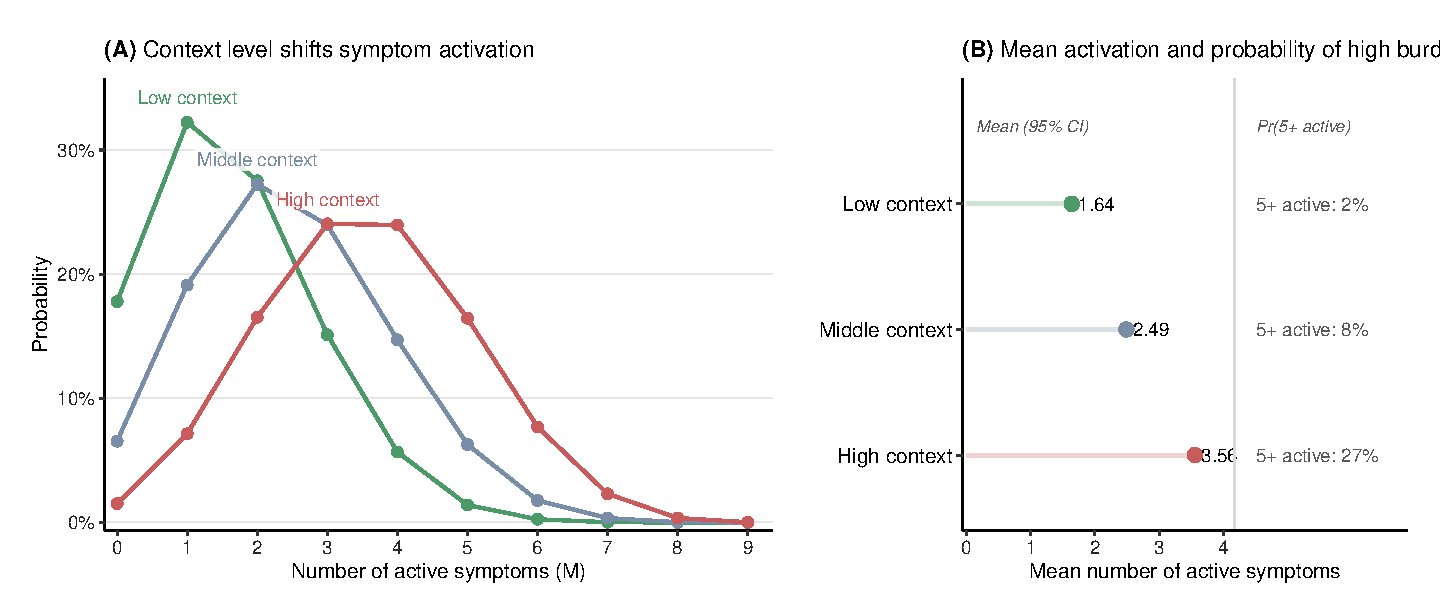
\includegraphics[width=\textwidth]{figs/revision_2026/Figure2_context_baseline.pdf}
\caption{\textbf{Slow contextual level shifts overall symptom activation under fixed symptom coupling.}
(A) The distribution of the number of active symptoms shifts toward higher activation as the slow contextual level \(P\) increases.
(B) Mean number of active symptoms and the probability of five or more active symptoms both increase across slow-context conditions.}
\label{fig:context-baseline}
\end{figure}


% ------------------------------------------------------------
% 6. Simulation 2 -- results (verified against sim2_summary.csv)
% ------------------------------------------------------------
\paragraph{Results.}
Before the perturbation, the slow field remained near its baseline
(\(P\approx 0.00\)), and the mean number of active symptoms was about
\(M=2.48\) out of 9. At shock onset, the slow field increased to approximately
\(P=1.00\). Symptom activation rose shortly afterward, reaching a peak of about
\(M=4.73\) active symptoms.

By the end of the recovery window, the slow field had returned close to
baseline (\(P\approx 0.06\)), and symptom activation had also largely recovered
(\(M\approx 2.58\)). Thus, an acute perturbation to the slow field produced a
temporary increase in symptom activation without changing the symptom--symptom
coupling matrix. In this simulation, persistence was limited because feedback
from symptoms to the slow field was turned off.


% ------------------------------------------------------------
% 7. Simulation 3 -- calibration-sentence fix, results (ADJUSTED to
%    cover all three current Figure 3 panels: A off/on, B shock-grid,
%    C history-dependence index), Figure 3 insert
% ------------------------------------------------------------
% Replace "This value was chosen from a small pilot grid because" with:
%   We used \(b=0.50\), a value that produced a visible delay in
%   recovery while all trajectories continued to decay toward baseline.

\paragraph{Results.}
Before the shock, both conditions were close to baseline. With feedback off,
the mean slow field during the last 50 pre-shock steps was approximately
\(P=-0.003\), and the mean number of active symptoms was \(M=2.50\). With
feedback on (\(b=0.50\)), the corresponding values were \(P=0.013\) and
\(M=2.52\).

The immediate post-shock response was similar across conditions, as expected.
In the first 20 post-shock steps, peak activation was \(M=4.34\) active
symptoms with feedback off and \(M=4.43\) with feedback on. The difference
emerged during recovery. By the end of the recovery window, the slow field had
nearly returned to baseline when feedback was off (\(P=0.05\)), but remained
higher when feedback was on (\(P=0.24\)). Symptom activation showed the same
pattern, returning to \(M=2.57\) with feedback off but remaining higher with
feedback on (\(M=2.89\)).

To ask whether this slowed recovery is simply a matter of degree or reflects a
qualitatively different regime, we repeated the same shock across a wider
range of feedback strengths (\(b=0, 0.50, 0.75, 1.00\)), holding every other
parameter fixed (Figure~\ref{fig:recovery-feedback}, panel B). Recovery
slowed progressively as \(b\) increased: mean symptom activation returned to
within about 0.01 of its pre-shock level by the end of the window at
\(b=0\) and \(b=0.50\), but at \(b=1.00\) it instead settled at a clearly
elevated plateau (\(m\approx0.49\), roughly double the pre-shock level of
\(m\approx0.28\)) that showed no sign of decaying further within the
simulated window.

This raised the question of whether the elevated \(b=1.00\) state reflects a
genuinely different equilibrium or is simply a slower version of the same
recovery. We tested this directly with an independent history-dependence
check (Figure~\ref{fig:recovery-feedback}, panel C): for each feedback
strength, we compared long trajectories started from a low-activation state to
trajectories started from a high-activation state, with no shock. Across
\(b=0\) to \(b=0.90\), late-window activation converged regardless of starting
state (separation in mean late activation \(\Delta m<0.15\) throughout, e.g.\
\(\Delta m=0.13\) at \(b=0.90\)). From \(b=1.00\) onward, however, the two
starting conditions remained separated (\(\Delta m=0.24\) at \(b=1.00\),
rising to a peak of \(\Delta m\approx0.52\) around \(b=1.4\)), and this
separation was not attributable to runaway growth in the slow field: the
largest slow-field excursion observed anywhere in this grid
(\(\max|P|\approx5.0\) at \(b=1.5\)) remained well below the threshold we used
to flag unbounded growth (\(|P|=6\)).

Together, these results show that symptom-to-context feedback does more than
slow recovery from a single perturbation. Beyond a threshold feedback
strength, the same slow--fast architecture becomes history-dependent: the
system no longer reliably returns to one baseline state, and its late symptom
activation instead depends on where it started. The feedback strength used in
the main simulations (\(b=0.50\)) falls within the convergent regime, so this
history-dependence is a property the model can exhibit under stronger
feedback, not an assumption built into the main results.

\begin{figure}[ht]
\centering
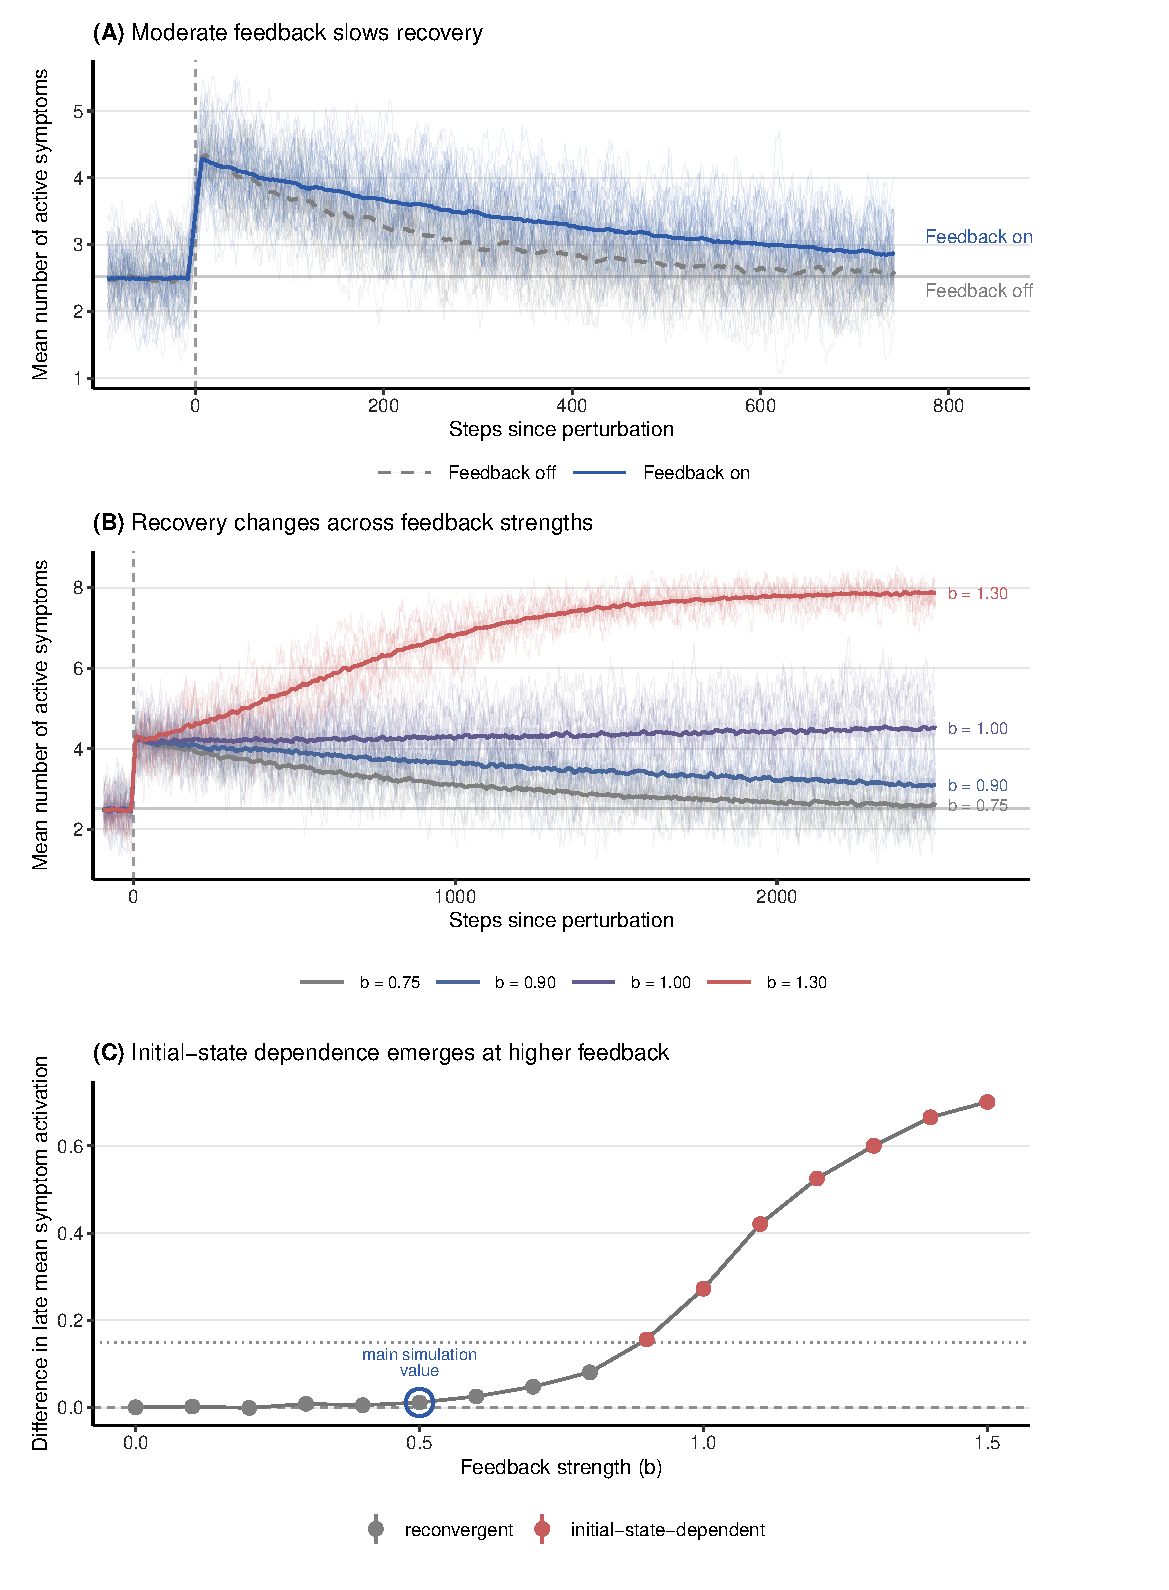
\includegraphics[width=\textwidth]{figs/revision_2026/Figure3_regimes.pdf}
\caption{\textbf{Feedback strength governs recovery and history-dependence in the slow--fast model.}
(A) Under the locked moderate-feedback level (\(b = 0.50\)), an acute perturbation to the slow contextual field is followed by a transient rise in mean symptom activation (\(m_t\)); trajectories recover toward baseline whether or not symptom-to-context feedback is present.
(B) Applying the same perturbation across a range of feedback strengths shows a shift from full recovery (\(b = 0\)) to settling at a stable, elevated plateau (\(b = 1.0\)), rather than returning to the pre-shock level.
(C) A history-dependence index summarizes, across the same feedback-strength range, whether late mean symptom activation depends on the system's initial state. Trajectories initialized from a low- versus a high-activation state converge under weaker feedback but remain separated once feedback strength exceeds approximately \(b = 1.0\) (history-dependent regime), while very high feedback strengths instead approach runaway growth in the slow field rather than a genuine second equilibrium. The locked main-text feedback level (\(b = 0.50\)) falls within the convergent regime.}
\label{fig:recovery-feedback}
\end{figure}


% ------------------------------------------------------------
% 8. Simulation 4 -- terminology fixes + figure placement (as given,
%    no Figure 3 conflict here)
% ------------------------------------------------------------
% Replace "mean absolute recovery error relative to the true coupling
% matrix" with "mean absolute edge-estimation error relative to the true
% coupling matrix". Replace every instance of "edge-recovery error" with
% "edge-estimation error". Replace "phantom edges" with "apparent edges
% among truly uncoupled symptom pairs" (or keep "phantom edges" but only
% after defining it once -- this also matches the orange phantom-edge
% highlighting now used in Figure 4 panels B/C).
%
% Cleaner metric sentence:
%   We compared estimated global strength, mean absolute edge-estimation
%   error relative to the true coupling matrix, and the number of
%   apparent edges above 0.10 among symptom pairs with no true direct
%   coupling.

\begin{figure}[ht]
\centering
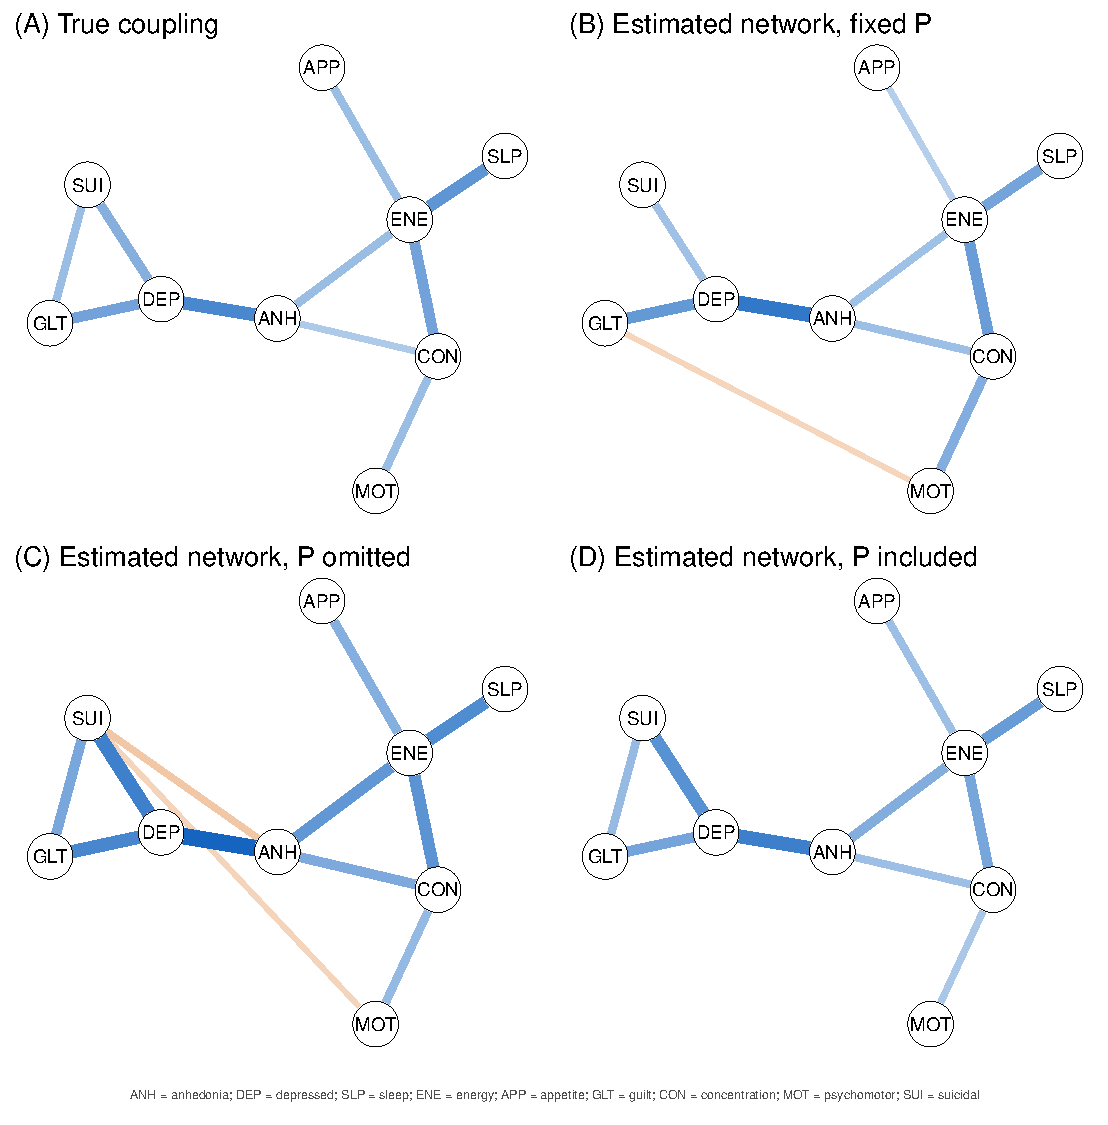
\includegraphics[width=\textwidth]{figs/revision_2026/Figure4_network_trio.pdf}
\vspace{0.75em}
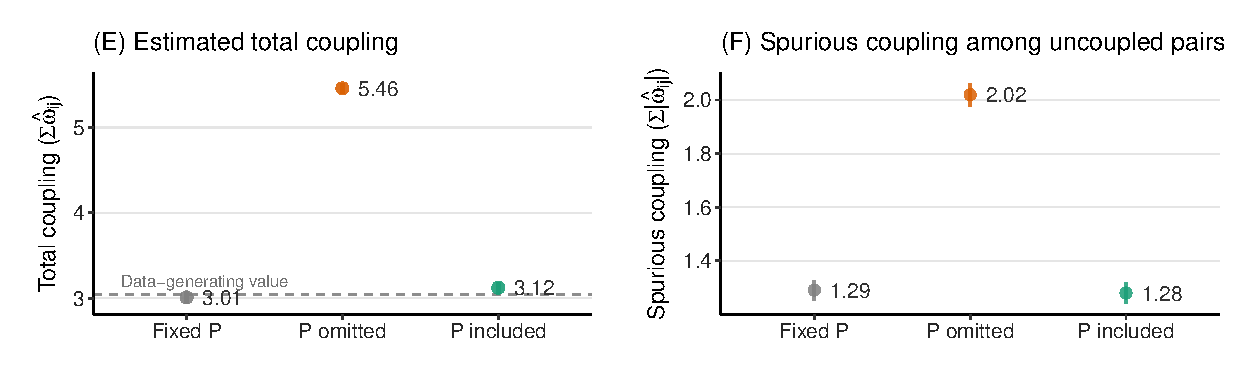
\includegraphics[width=0.82\textwidth]{figs/revision_2026/Figure4_metric_strip.pdf}
\caption{\textbf{Omitting slow context makes estimated symptom networks look more connected.}
(A) True symptom--symptom coupling matrix used to generate the data.
(B) Network estimated from pooled symptom profiles when the slow contextual field varies across people but is omitted from the estimator. Orange edges mark phantom couplings: connections absent in the true network that nonetheless appear in this estimate.
(C) Network estimated from the same pooled data after including the slow contextual field as a covariate; the same phantom-edge coloring is applied, and few or no orange edges remain.
(D) Omitting \(P\) produces the largest excess estimated global strength relative to the true coupling matrix.
(E) Error on truly absent edges is also largest when \(P\) is omitted, indicating more apparent coupling among symptom pairs with no true direct edge. Points and intervals in panels D--E show means and standard errors across 30 independent replicates.}
\label{fig:network-estimation}
\end{figure}


% ------------------------------------------------------------
% 9. Discussion (ADJUSTED: history-dependence gets its own subsection,
%    stated as a direct main-text finding, not a hedged supplementary
%    aside -- since it's now Figure 3 panel C, not a separate Figure S)
% ------------------------------------------------------------
\section{Discussion}

\subsection{Main contribution}
We developed a computational slow--fast model in which a fast symptom network
is embedded in a slower contextual field. The model keeps symptom-specific
activation tendencies, symptom--symptom coupling, and slow contextual input
separate. This separation matters because the same observed symptom pattern
can reflect different combinations of fast coupling and slow context.

\subsection{Slow context changes activation without changing coupling}
Simulation 1 showed that the same fixed symptom--symptom coupling matrix can
produce systematically different activation distributions depending on the
slow contextual baseline it is embedded in. This is the simplest version of
the paper's central claim: differences in observed symptom activation do not,
by themselves, imply differences in how symptoms are coupled to one another.

\subsection{Feedback can slow recovery}
Simulations 2 and 3 showed that an acute perturbation to the slow field
produces a temporary rise in symptom activation followed by recovery, and that
feedback from sustained symptom activation back into the slow field slows this
recovery. At the feedback strength used in the main simulations, the system
still recovered -- feedback changed the timescale of recovery, not its
eventual outcome.

\subsection{History-dependence under stronger feedback}
Extending the same shock design across a wider range of feedback strengths
(Figure~\ref{fig:recovery-feedback}, panels B--C) showed that slower recovery
is a matter of degree only up to a point. Beyond a threshold feedback
strength (here, around \(b\approx1.0\)), trajectories starting from different
initial states no longer converge to the same late state, indicating a
qualitatively different, history-dependent regime rather than merely slower
recovery. This history-dependence emerged directly from the heterogeneous,
symptom-level architecture used throughout this paper, without reintroducing
the homogeneous mean-field approximation used in earlier work. We treat it as
a genuine regime of the revised model, not a supplementary curiosity, though
the feedback strengths at which it appears are stronger than the value used in
the main simulations, and its correspondence to any specific clinical
phenomenon (e.g., diagnostic transitions, relapse) remains an open question
for future work.

\subsection{When context looks like coupling}
Simulation 4 showed that omitting the slow contextual field from an estimated
symptom network inflated apparent connectivity, including apparent edges
between symptom pairs with no true direct coupling. Including the slow field
as a covariate reduced this inflation. This suggests that some of what
network models attribute to symptom--symptom coupling may instead reflect
shared dependence on an unmeasured slow context.

\subsection{Limitations}
Several limitations should temper how these results are interpreted. The
simulations are theoretical and are not calibrated to a specific clinical
population. The slow contextual field is one-dimensional, and symptom states
are binary, both simplifications relative to real symptom measurement.
Symptom--symptom couplings in these examples are positive only. Parameter
choices throughout are illustrative rather than fitted to data. The
context-adjusted estimator used in Simulation 4 corrects for a specific,
known confound in this simulation and is not a general causal identification
strategy. Finally, the history-dependent regime identified here has not been
validated against real longitudinal transitions and should not yet be
interpreted as evidence for clinical tipping points.

\subsection{Conclusion}
Fast psychological states do not unfold in isolation from slower contextual
conditions. By embedding a symptom-level network in a slower contextual
field, the present model shows how slow context can shift activation, shape
recovery, prolong persistence through feedback, produce history-dependent
regimes under stronger feedback, and alter the interpretation of estimated
symptom networks. The main implication is not that symptom--symptom coupling
is unimportant, but that coupling and context need to be modeled together
when interpreting psychological dynamics.
